\documentclass{article}

\usepackage[margin=1in]{geometry} % Set margins to 1 inch
\usepackage{graphicx} % Allows including images
\usepackage{float} % Allows for precise placement of figures
\usepackage{amsmath} % Allows for math equations
\usepackage{siunitx} % Allows for SI units
\usepackage{placeins} % Makes sure images are in their respective sections by \FloatBarrier

\begin{document}

\title{Hardware Assignment Report}
\author{Anagha Balaji \\ EE22BTECH11204}
\date{}
\maketitle

\section{Aim}
To make a Random Number Generator using Shift Generators

\section{Components}
\begin{enumerate}    
    \item Breadboard
    \item Seven Segment Display : Common Anode
    \item Decoder [7447]
    \item FlipFlop [7474] x2
    \item XOR gate [7486]
    \item 555 IC
    \item Resistors [10M$\Omega$, 1K$\omega$ x2]
    \item Capacitors [47nF,470nF]
    \item USB micro B breakout board
    \item Jumper wires
\end{enumerate}

\begin{figure}[ht]
        \centering
        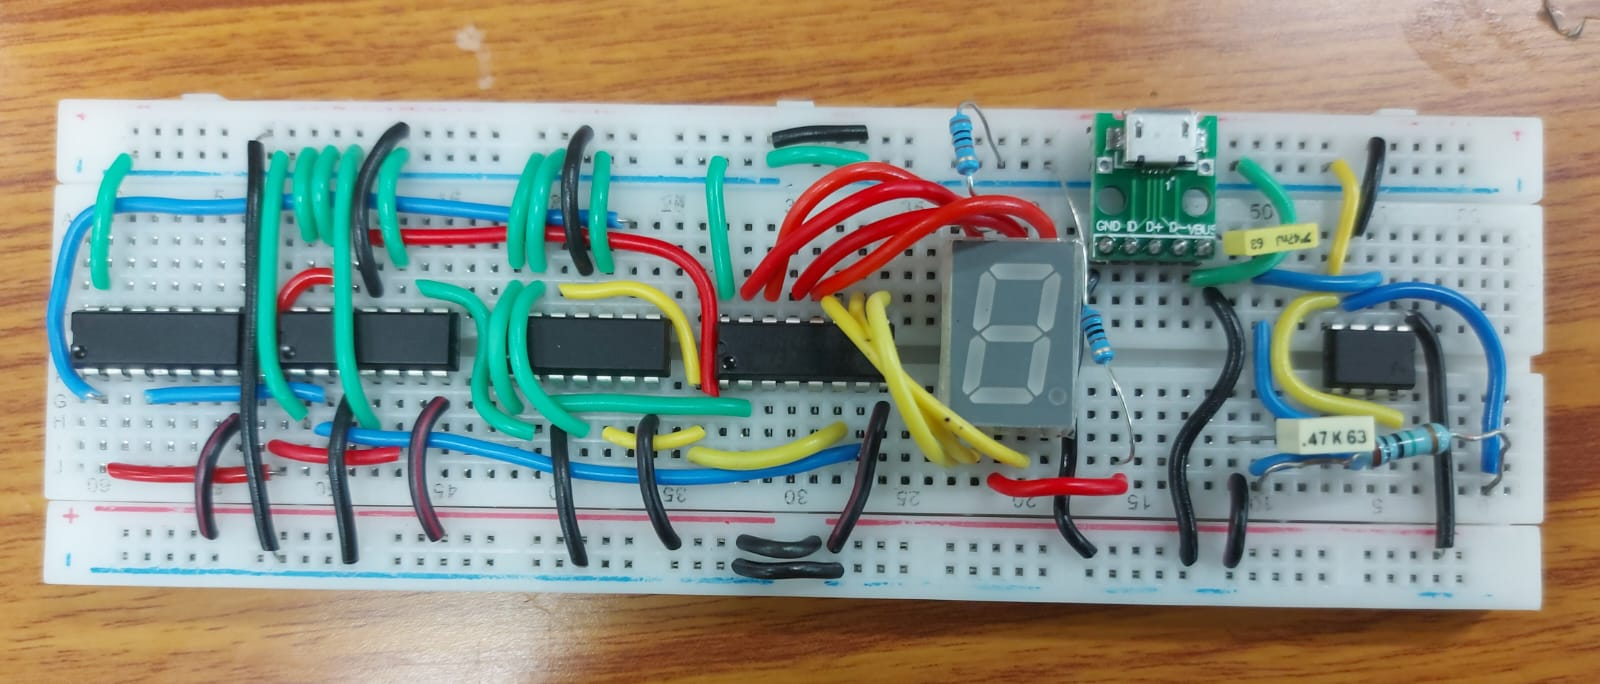
\includegraphics[width=1\linewidth]{hardware.jpeg}
        \caption{Circuit Board}
        \label{fig:view}
\end{figure}

\section{Description}
The given circuit is a visual representation of how randon variables can be connected to signal processing.
When considering the usage of a circuit with a seven-segment display in relation to random variables, it typically involves generating random numbers and displaying them on the seven-segment display. Random variables are variables whose values are determined by chance or probability.

\subsection{Seven segment Display}
Seven segment displays are the output display device that provides a way to display information in the form of images or text or decimal numbers.A circuit containing a seven-segment display is commonly used to visually represent numerical information. Each segment in the display corresponds to a specific digit from 0 to 9, and by selectively activating or deactivating these segments, various numbers can be shown.

\subsection{Decoder}
The combinational circuit that change the binary information into $2^N$ output lines is known as Decoders. The binary information is passed in the form of N input lines. The output lines define the $2^N$-bit code for the binary information. In simple words, the Decoder performs the reverse operation of the Encoder. At a time, only one input line is activated for simplicity. The produced $2^N$-bit output code is equivalent to the binary information.

\subsection{Flip Flop}
A circuit that has two stable states is treated as a flip flop. These stable states are used to store binary data that can be changed by applying varying inputs. The flip flops are the fundamental building blocks of the digital system. Flip flops and latches are examples of data storage elements. In the sequential logical circuit, the flip flop is the basic storage element. The latches and flip flops are the basic storage elements but different in working.

\subsection{555 IC}
The 555 timer IC is an integrated circuit  used in a variety of timer, delay, pulse generation, and oscillator applications.useful precision timing device which can act as either a simple timer to generate single pulses or long time delays, or as a relaxation oscillator producing a string of stabilised waveforms of varying duty cycles from 50 to 100.

\subsection{Overview}
The Flip Flofs take the input and based on that outputs are generated. The generated outputs are random and the numbers shown are from 1 to 15. The randomness is predictable because this system is deterministic.a deterministic system is a system in which no randomness is involved in the development of future states of the system.\\
The order of the output in this case follows : 1, 3, 7, 15, 14, 13, 10, 5, 11, 6, 12, 9, 2, 4, 8

\section{Block Diagram}
\begin{figure}[ht]
        \centering
        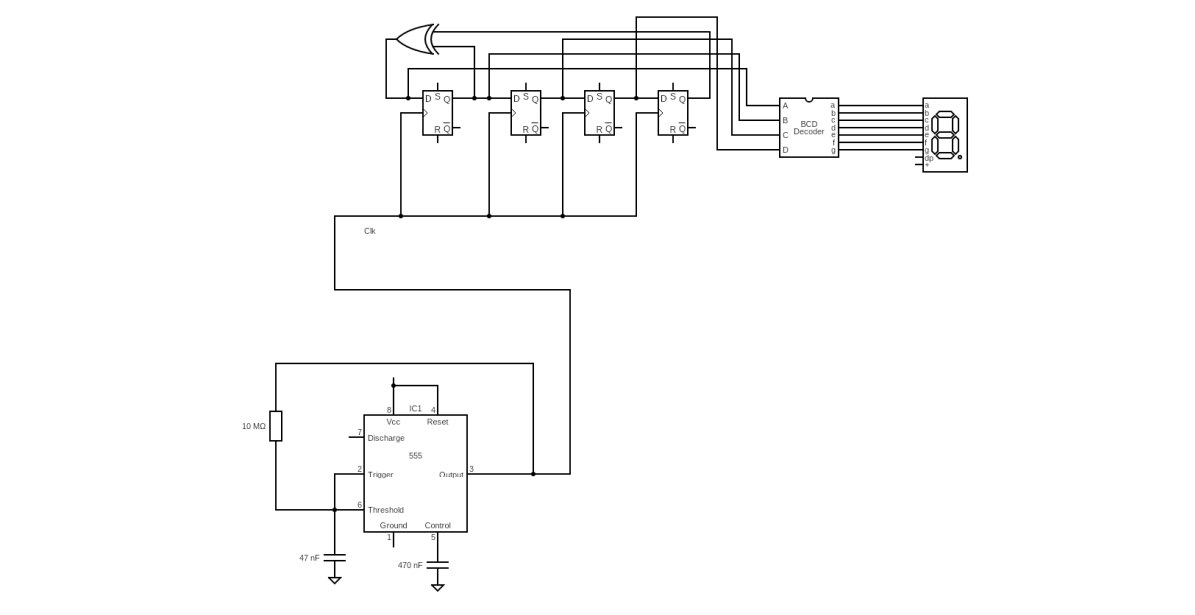
\includegraphics[width=0.8\linewidth]{hardware1.jpg}
        \caption{Block Diagram}
        \label{fig:view}
\end{figure}

\end{document}
